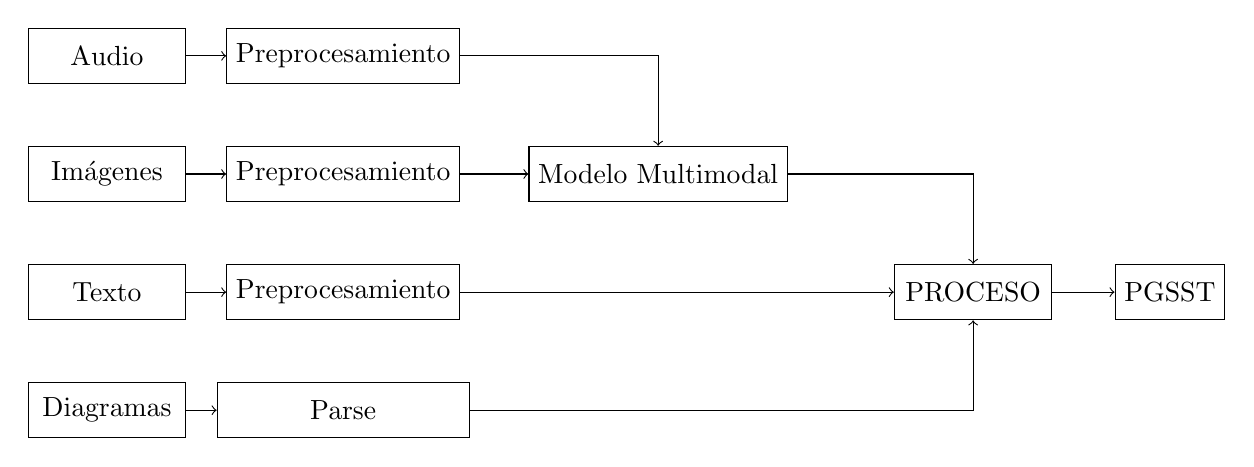
\begin{tikzpicture}[node distance=2cm and 3cm, every node/.style={draw, rectangle, minimum height=2em, minimum width=2cm, align=center}]

    % Nodes
    \node (img) {Imágenes};
    \node (txt) [below of=img, node distance=1.5cm] {Texto};
    \node (grf) [below of=txt, node distance=1.5cm] {Diagramas};
    \node (audio) [above of=img, node distance=1.5cm] {Audio};

    \node (preprocess1) [right of=img, node distance=3cm] {Preprocesamiento};
    \node (preprocess2) [right of=txt, node distance=3cm] {Preprocesamiento};
    \node (preprocess3) [right of=audio, node distance=3cm] {Preprocesamiento};
    
    \node (multim) [right of=preprocess1, node distance=4cm] {Modelo Multimodal};
    \node (parse) [right of=grf, node distance=3cm, minimum width=3.2cm] {Parse};

    \node (process) [right of=txt, xshift=9cm, minimum height=2em] {PROCESO};
    \node (pgsst) [right of=process, node distance=2.5cm, minimum width=1cm] {PGSST};

    % Arrows
    \draw[->] (img) -- (preprocess1);
    \draw[->] (preprocess1) -- (multim);

    \draw[->] (txt) -- (preprocess2);
    \draw[->] (preprocess2) -- (process);
    
    \draw[->] (process) -- (pgsst);

    \draw[->] (multim) -| (process);
    
    \draw[->] (grf) -- (parse);
    \draw[->] (parse) -| (process);

    \draw[->] (audio) -- (preprocess3);
    \draw[->] (preprocess3) -| (multim);

\end{tikzpicture}